

\section {Introduction}

\begin{frame}{Introduction}
  Les drones trouvent de nombreuses utilisations tant ludiques que professionnelles. Cet article présente un cas d'utilisation dans les télécommunications où le drone permettrait d'améliorer la qualité de service (QoS) ou de rétablir des communications après une catastrophe naturelle. 
 
 
\end{frame}


\begin{frame}{Contexte de l'article}
\begin{itemize}
	
	\item Date de première publication le 12 Janvier 2018.
	
	\item Publié aussi dans le journal IEEE Transactions on Wireless Communications 
	( Volume: 17 , Issue: 4 , April 2018 ) qui s'adresse à un public intéressé par les communications sans fils.
	
	\item Article visant un objectif essentiellement concret
	\item Bibliographie effectuée : Etat de l'art dans les domaines relatifs aux UAV, Articles plus théoriques sur 
	la résolution du TSP notamment publiés par "l'European Journal of Operational Research",
	ou par "Cambridge Univ. Press".
	\item Financé par l'Université de Singapour.
	
\end{itemize}
\end{frame}
 
\begin{frame}{Dissémination multicast sans fil d'un message}

Le présent article étudie un drone déployé en vue de disséminer vers des Terminaux Terrestres (GT) un message via une connexion sans fil. On parle de multicast, et non de broadcast, car à un instant donné seule une partie des GT est à portée du drone.

\begin{figure}
	\centering
	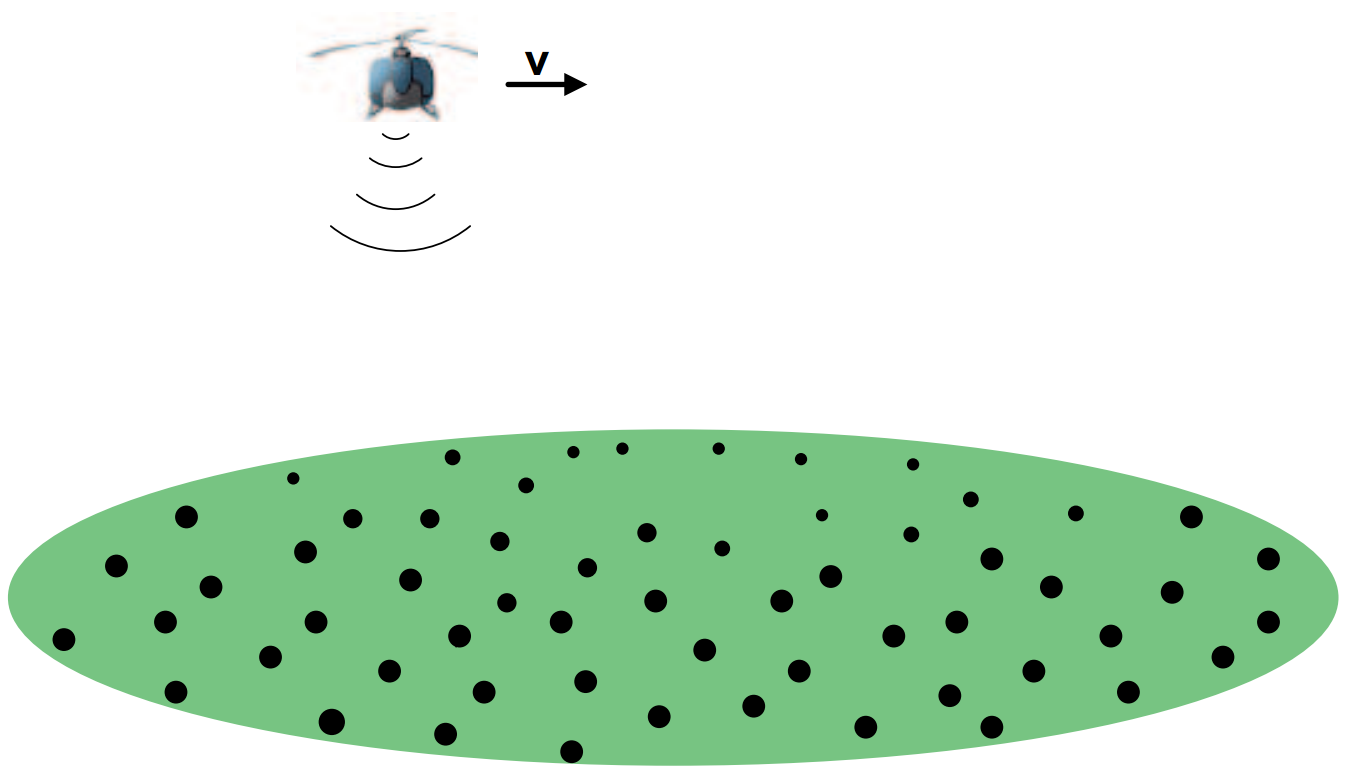
\includegraphics[width=0.7\linewidth]{images/multicast}
	\caption{}
	\label{fig:multicast}
\end{figure}

\end{frame}

\begin{frame}{Minimisation du temps de mission et distance critique D}
Les auteurs cherchent à minimiser le temps de mission tout en assurant une réception du message par les GT avec une probabilité cible fixée à l'avance. Le tout sous la contrainte de vitesse maximale du drone. La probabilité de réception d'un GT est difficile à évaluer car c'est fonction compliquée de la trajectoire du drone. Pour contourner le problème, les auteurs reformulent le problème en introduisant un paramètre auxiliaire D (distance critique horizontale entre le drone et la GT). Au delà de cette distance D, le nombre de paquets perdus devient trop important car le temps de connexion devient insuffisant. 


\end{frame}


\newcounter{sauvegardeenumi}
\newcommand{\asuivre}{\setcounter{sauvegardeenumi}{\theenumi}}
\newcommand{\suite}{\setcounter{enumi}{\thesauvegardeenumi}}

\begin{frame}{Introduction}
	Ainsi les auteurs ont suivi le plan suivant : 
\begin{enumerate}
	
	\item Reformulation du problème en utilisant une seule contrainte
	de temps minimum de connexion entre le drone et le terminal terrestre.	
	\item Démonstration du théorème : " la trajectoire optimale
	peut-être constituée uniquement de segments de droites reliant des
	waypoints dont la position est optimisée."

	
\end{enumerate}
\asuivre
\end{frame}



\begin{frame}{Introduction}
 
\begin{enumerate}
	\suite
	\item Utilisation du concept de "stations de base virtuelles" (VBS) pour calculer ces waypoints ;  problème qui est en fait un TSP généralisé (NP-Hard).

	\item Optimisation de la vitesse en fonction du temps le long de la trajectoire obtenue
	en utilisant la programmation linéaire (LP).

\end{enumerate}

\end{frame}


\begin{frame}{Plan}
\tableofcontents
\end{frame}